\section{Related Work}
\begin{frame}{Related Work}
  \begin{figure}
    \centering
    \begin{tikzpicture}[scale=.35, node distance=3cm]
      \node [component] (extraction) {Keyphrase Extraction};
      \node [component, right=of extraction] (assignment) {Keyphrase Assignment};
  
      \node [io, above=of extraction] (document) {document};
      \node [io, above=of assignment] (controlled_vocabulary) {controlled vocabulary};
  
      \node [io, below=of extraction] (extracted_keyphrases) {keyphrases $\subseteq$ document};
      \node [io, below=of assignment] (assigned_keyphrases) {keyphrases $\subseteq$ controlled vocabulary};
  
      \node [above=of document, yshift=-2.85cm] (document_centric) {\small document-centric};
  
      \draw [dashed] ($(extraction.north west)+(-.5cm, 5.5cm)$) rectangle ($(extraction.south east)+(.5cm, -5.5cm)$);
      \node [above=of controlled_vocabulary, yshift=-2.9cm] (domain_specific) {\small domain-specific};
  
      \draw [dashed] ($(assignment.north west)+(-1cm, 5.5cm)$) rectangle ($(assignment.south east)+(1cm, -5.5cm)$);
  
      \path [->] (document) edge (extraction);
      \path [->] (extraction) edge (extracted_keyphrases);
      \path [->] (document) edge (assignment);
      \path [->] (controlled_vocabulary) edge (assignment);
      \path [->] (assignment) edge (assigned_keyphrases);
    \end{tikzpicture}
  \end{figure}
\end{frame}

\begin{frame}{Related Work}
  \begin{figure}
    \centering
    \begin{tikzpicture}[scale=.35, node distance=3cm]
      \node [selectedcomponent] (extraction) {Keyphrase Extraction};
      \node [component, right=of extraction] (assignment) {Keyphrase Assignment};
  
      \node [io, above=of extraction] (document) {document};
      \node [io, above=of assignment] (controlled_vocabulary) {controlled vocabulary};
  
      \node [io, below=of extraction] (extracted_keyphrases) {keyphrases $\subseteq$ document};
      \node [io, below=of assignment] (assigned_keyphrases) {keyphrases $\subseteq$ controlled vocabulary};
  
      \node [above=of document, yshift=-2.85cm] (document_centric) {\small document-centric};
  
      \draw [dashed, color=linared] ($(extraction.north west)+(-.5cm, 5.5cm)$) rectangle ($(extraction.south east)+(.5cm, -5.5cm)$);
      \node [above=of controlled_vocabulary, yshift=-2.9cm] (domain_specific) {\small domain-specific};
  
      \draw [dashed] ($(assignment.north west)+(-1cm, 5.5cm)$) rectangle ($(assignment.south east)+(1cm, -5.5cm)$);
  
      \path [->] (document) edge (extraction);
      \path [->] (extraction) edge (extracted_keyphrases);
      \path [->] (document) edge (assignment);
      \path [->] (controlled_vocabulary) edge (assignment);
      \path [->] (assignment) edge (assigned_keyphrases);
    \end{tikzpicture}
  \end{figure}
\end{frame}

\begin{frame}{Related Work}\framesubtitle{Keyphrase extraction}
  \begin{block}{Supervised keyphrase extraction}
    \begin{itemize}
      \item{Relying on reference keyphrases}
      \item{Learning to determine keyphrase likelihood}
      \item{Mixing statistical and linguistic features}
    \end{itemize}
  \end{block}
  
  \begin{block}{Unsupervised keyphrase extraction}
    \begin{itemize}
      \item{Looking for the most important keyphrase candidates}
      \item{Using mainly statistics}
      \item{Linking keyphrase candidates to each other}
    \end{itemize}
  \end{block}
\end{frame}

\begin{frame}{Related Work}\framesubtitle{Keyphrase extraction (TopicRank)}\vspace{.5em}
  Graph-based approach detecting documents most important topics and extracting keyphrases from these topics
  
  \vspace{.75em}
  
  \begin{enumerate}
    \item{Keyphrase candidate selection\hfill{}\uncover<2->{\texttt{/(NOUN | ADJ)+/}}}
    \item{Keyphrase candidates topical clustering\hfill{}\uncover<3->{\textit{lexical clustering}}}
    \item{Topic graph construction\hfill{}\uncover<4->{\textit{complete graph}}}
    \item{Graph-based topic ranking\hfill{}\uncover<5->{\textit{Google's PageRank}}}
    \item{Keyphrase extraction from the important topics\hfill{}\uncover<6->{\textit{one per topic}}}
  \end{enumerate}
  
  \vspace{.5em}
  
  \begin{center}
    \begin{tikzpicture}[scale=.4,
                        align=center,
                        every node/.style={transform shape},
                        main node/.style={text centered,
                                          circle,
                                          draw=black,
                                          fill=white,
                                          minimum width=1.2cm,
                                          inner sep=1.5pt,
                                          font=\Large\bfseries}]
      \visible<3->{
          \foreach \number/\pos in {1/above,2/above,3/above,4/above,5/above,6/above,7/above,8/above,9/above,10/above,11/below,12/below,13/below,14/below,15/below,16/below,17/below,18/below,19/below}{
            \mycount=\number
            \advance\mycount by -1
            \multiply\mycount by 19
            \advance\mycount by 0
            \ifthenelse{\number > 9}{
              \node[main node] (N-\number) at (\the\mycount:5cm) {$t_{\number}$};
            }{
              \node[main node] (N-\number) at (\the\mycount:5cm) {$~t_{\number}~$};
            }
          }
      }
      \visible<4->{
          \foreach \number in {1,...,18}{
            \mycount=\number
            \advance\mycount by 1
            \foreach \numbera in {\the\mycount,...,19}{
              \path[black!50] (N-\number) edge (N-\numbera);
            }
          }
          \path[black!75, line width=.7mm] (N-1) edge (N-11);
          \path[black!75, line width=.5mm] (N-1) edge (N-12);
          \path[black!75, line width=.2mm] (N-2) edge (N-7);
          \path[black!75, line width=1mm] (N-6) edge (N-14);
          \path[black!75, line width=1mm] (N-6) edge (N-17);
          \path[black!75, line width=.4mm] (N-6) edge (N-19);
          \path[black!75, line width=.2mm] (N-7) edge (N-12);
          \path[black!75, line width=.2mm] (N-9) edge (N-16);
          \path[black!75, line width=.4mm] (N-12) edge (N-19);
      }
      \visible<3->{
          \foreach \number/\pos in {1/above,2/above,3/above,4/above,5/above,6/above,7/above,8/above,9/above,10/above,11/below,12/below,13/below,14/below,15/below,16/below,17/below,18/below,19/below}{
            \mycount=\number
            \advance\mycount by -1
            \multiply\mycount by 19
            \advance\mycount by 0
            \ifthenelse{\number > 9}{
              \node[main node] (N-\number) at (\the\mycount:5cm) {$t_{\number}$};
            }{
              \node[main node] (N-\number) at (\the\mycount:5cm) {$~t_{\number}~$};
            }
          }
      }
      \visible<5->{
          \foreach \number/\pos in {1/above,2/above,3/above,4/above,5/above,6/above,7/above,8/above,9/above,10/above,11/below,12/below,13/below,14/below,15/below,16/below,17/below,18/below,19/below}{
            \mycount=\number
            \advance\mycount by -1
            \multiply\mycount by 19
            \advance\mycount by 0
            \ifthenelse{\number = 12}{
                \node[main node, draw=linared, line width=.5mm, fill=white] (N-\number) at (\the\mycount:5cm) {\textcolor{linared}{\textbf{$t_{\number}$}}};
            }{
                \ifthenelse{\number = 1}{
                    \node[main node, draw=linared, line width=.5mm, fill=white] (N-\number) at (\the\mycount:5cm) {\textcolor{linared}{\textbf{$~t_{\number}~$}}};
                }{
                    \ifthenelse{\number = 17}{
                        \node[main node, draw=linared, line width=.5mm, fill=white] (N-\number) at (\the\mycount:5cm) {\textcolor{linared}{\textbf{$t_{\number}$}}};
                    }{
                        \ifthenelse{\number = 14}{
                            \node[main node, draw=linared, line width=.5mm, fill=white] (N-\number) at (\the\mycount:5cm) {\textcolor{linared}{\textbf{$t_{\number}$}}};
                        }{
                            \ifthenelse{\number = 6}{
                                \node[main node, draw=linared, line width=.5mm, fill=white] (N-\number) at (\the\mycount:5cm) {\textcolor{linared}{\textbf{$~t_{\number}~$}}};
                            }{
                                \ifthenelse{\number > 9}{
                                  \node[main node] (N-\number) at (\the\mycount:5cm) {$t_{\number}$};
                                }{
                                  \node[main node] (N-\number) at (\the\mycount:5cm) {$~t_{\number}~$};
                                }
                            }
                        }
                    }
                }
            }
          }
      }
    \end{tikzpicture}
  \end{center}
\end{frame}

\begin{frame}{Related Work}\framesubtitle{Keyphrase extraction (TopicRank -- Example)}
  \vfill{}
  \begin{exampleblock}{\normalsize
    \textit{Toucher~: le tango des sens. Problèmes de \textbf{sémantique lexicale}}
  }\justifying\footnotesize
    \textit{À partir d'une hypothèse sur la sémantique de l'unité lexicale `toucher' formulée en termes de forme schématique, cette étude vise à rendre compte de la \textbf{variation sémantique} manifestée par les emplois de ce \textbf{verbe} dans la construction \textbf{transitive} directe `C0 toucher C1'. Notre étude cherche donc à articuler variation sémantique et invariance fonctionnelle. Cet article concerne essentiellement le mode de variation co-textuelle~: en conséquence, elle ne constitue qu'une première étape dans la compréhension de la construction des valeurs référentielles que permet 'toucher'. Une étude minutieuse de nombreux exemples nous a permis de dégager des constantes impératives sous la forme des 4 notions suivantes~: sous-détermination sémantique, contact, anormalité, et contingence. Nous avons tenté de montrer comment ces notions interprétatives sont directement dérivables de la forme schématique proposée.}
  
    \begin{exampleblock}{\normalsize Reference keyphrases (French):}
      \textit{Français}; \textit{modélisation}; \textit{analyse distributionnelle}; \textit{interprétation sémantique}; \textbf{\textit{variation sémantique}}; \textbf{\textit{transitif}}; \textbf{\textit{verbe}}; \textit{syntaxe}; \textbf{\textit{sémantique lexicale}}.
    \end{exampleblock}
    
    \vspace{-.75em}
    
    \begin{exampleblock}{\normalsize \textbf{TopicRank 10 keyphrases (French):}}
      \underline{\textit{Sémantique lexicale}};
      \underline{\textit{variation sémantique}};
      \textit{problèmes};
      \textit{étude};
      \textit{forme schématique};
      \textit{sens};
      \textit{tango};
      \textit{invariance fonctionnelle};
      \textit{construction transitive directe};
      \textit{article};
    \end{exampleblock}
  \end{exampleblock}
  \vfill{}
\end{frame}

\begin{frame}{Related Work}
  \begin{figure}
    \centering
    \begin{tikzpicture}[scale=.35, node distance=3cm]
      \node [component] (extraction) {Keyphrase Extraction};
      \node [selectedcomponent, right=of extraction] (assignment) {Keyphrase Assignment};
  
      \node [io, above=of extraction] (document) {document};
      \node [io, above=of assignment] (controlled_vocabulary) {controlled vocabulary};
  
      \node [io, below=of extraction] (extracted_keyphrases) {keyphrases $\subseteq$ document};
      \node [io, below=of assignment] (assigned_keyphrases) {keyphrases $\subseteq$ controlled vocabulary};
  
      \node [above=of document, yshift=-2.85cm] (document_centric) {\small document-centric};
  
      \draw [dashed] ($(extraction.north west)+(-.5cm, 5.5cm)$) rectangle ($(extraction.south east)+(.5cm, -5.5cm)$);
      \node [above=of controlled_vocabulary, yshift=-2.9cm] (domain_specific) {\small domain-specific};
  
      \draw [dashed, color=linared] ($(assignment.north west)+(-1cm, 5.5cm)$) rectangle ($(assignment.south east)+(1cm, -5.5cm)$);
  
      \path [->] (document) edge (extraction);
      \path [->] (extraction) edge (extracted_keyphrases);
      \path [->] (document) edge (assignment);
      \path [->] (controlled_vocabulary) edge (assignment);
      \path [->] (assignment) edge (assigned_keyphrases);
    \end{tikzpicture}
  \end{figure}
\end{frame}

\begin{frame}{Related Work}\framesubtitle{Keyphrase assignment}
  \begin{itemize}
    \item{Relying on a domain-specific controlled vocabulary (thesaurus)}
    \item{Aiming for consistency across domain}
    %\item{Using a supervised approach}
  \end{itemize}
  
  \vfill{}
  
  \uncover<2->{
    \begin{center}
      \textbf{Handful of attempts}
    \end{center}
  }
\end{frame}

\begin{frame}{Related Work}\framesubtitle{Keyphrase assignment (KEA++)}
  \begin{center}
    \vspace{-1em}
    \alt<3>{
      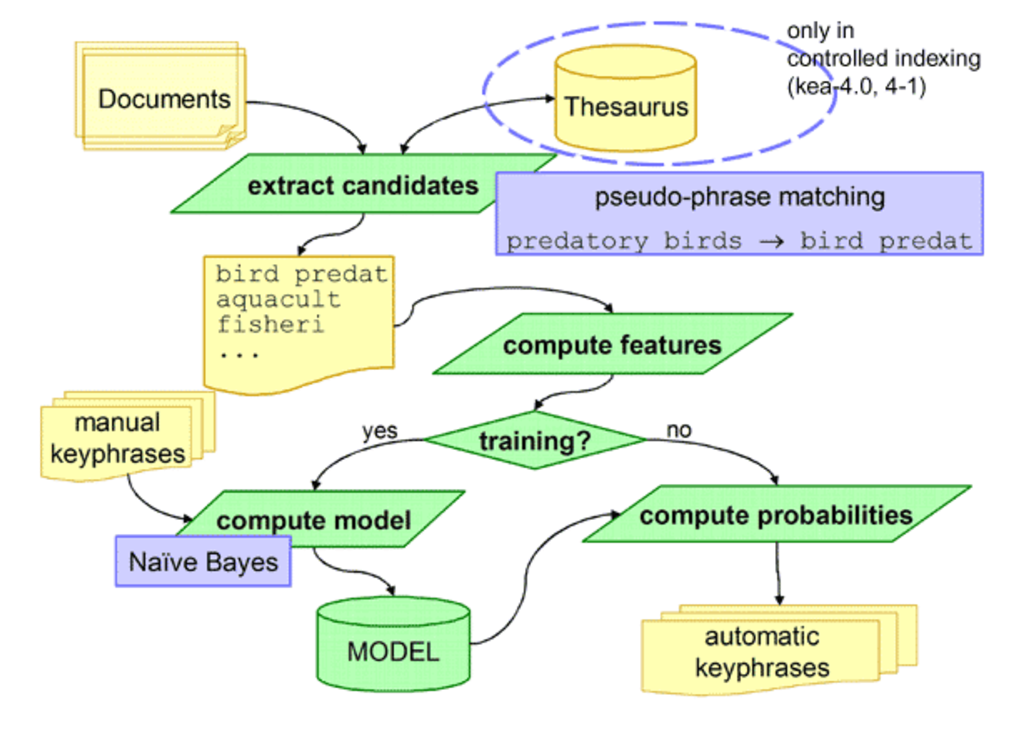
\includegraphics[height=.85\textheight]{pictures/kea_diagram.eps}
    }{
      \alt<2>{
        \includegraphics[height=.85\textheight]{pictures/kea_diagram_2.eps}
      }{
        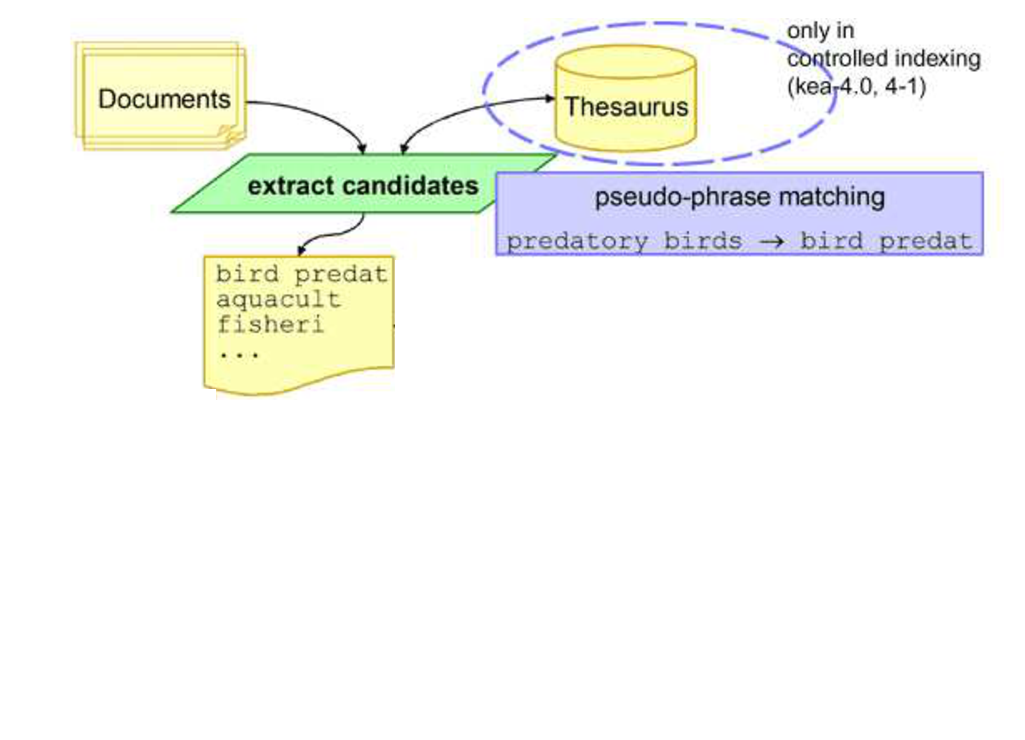
\includegraphics[height=.85\textheight]{pictures/kea_diagram_1.eps}
      }
    }
    \vspace{.25em}
    Figure from \cite{medelyan2006kea++}
  \end{center}
\end{frame}

\begin{frame}{Related Work}\framesubtitle{Keyphrase extraction (KEA++ -- Example)}
  \vfill{}
  \begin{exampleblock}{\normalsize
    \textit{Toucher~: le tango des sens. Problèmes de \textbf{sémantique lexicale}}
  }\justifying\footnotesize
    \textit{À partir d'une hypothèse sur la sémantique de l'unité lexicale `toucher' formulée en termes de forme schématique, cette étude vise à rendre compte de la \textbf{variation sémantique} manifestée par les emplois de ce \textbf{verbe} dans la construction \textbf{transitive} directe `C0 toucher C1'. Notre étude cherche donc à articuler variation sémantique et invariance fonctionnelle. Cet article concerne essentiellement le mode de variation co-textuelle~: en conséquence, elle ne constitue qu'une première étape dans la compréhension de la construction des valeurs référentielles que permet 'toucher'. Une étude minutieuse de nombreux exemples nous a permis de dégager des constantes impératives sous la forme des 4 notions suivantes~: sous-détermination sémantique, contact, anormalité, et contingence. Nous avons tenté de montrer comment ces notions interprétatives sont directement dérivables de la forme schématique proposée.}
  
    \begin{exampleblock}{\normalsize Reference keyphrases (French):}
      \textit{Français}; \textit{modélisation}; \textit{analyse distributionnelle}; \textit{interprétation sémantique}; \textbf{\textit{variation sémantique}}; \textbf{\textit{transitif}}; \textbf{\textit{verbe}}; \textit{syntaxe}; \textbf{\textit{sémantique lexicale}}.
    \end{exampleblock}
    
    \vspace{-.75em}
    
    \begin{exampleblock}{\normalsize \textbf{Kea$++$ 10 keyphrases (French):}}
      \textit{Toucher};
      \underline{\textit{variation sémantique}};
      \textit{sémantique};
      \textit{tangoa};
      \textit{direction};
      \textit{formant};
      \underline{\textit{sémantique lexicale}};
      \textit{impératif};
      \textit{invariant sémantique};
      \textit{transitif};
    \end{exampleblock}
  \end{exampleblock}
  \vfill{}
\end{frame}

\begin{frame}{Related Work}
  \begin{center}
    \begin{tabular}{rcl}
      \textbf{Extraction} & \underline{\textbf{Vs.}} & \textbf{Assignment}\\
      & & \\
      Leveraging document content & \underline{Vs.} & Ignoring inner-document relations\\
      Ignoring domain vocabulary & \underline{Vs.} & Mapping document to its domain\\
      Limited to document content & \underline{Vs.} & Limited to vocabulary coverage
    \end{tabular}
  \end{center}
  
  \vfill{}
  
  \begin{block}<2->{Professional indexer point of view}
    Annotated keyphrases should respect the vocabulary of the domain as much as possible, but should not be restricted to it in order to be exhaustive.
  \end{block}
\end{frame}
